\documentclass{article}

\usepackage{tikz}
\usepackage{physics}

\begin{document}
\title{Quantum computer architecture}
 \author{John Scott, Oliver Thomas}
\maketitle

\abstract{This is for a demonstration of 12 or 16 \textit{Classical qubits} to
    demonstrate the differences between a 4 bit digital microcomputer and state of the
art quantum processors}

\section{Notes about the electronic design}

\begin{itemize}
    \item 16 qubits (4 by 4 grid) requires $2^{16}=65536$ entries in the state vector. Each entry must be signed and could optionally be complex (to express the addition algorithm). If we used 4 bits of precision that means complex amplitudes require 16bits. Then the state vector can be stored in 131072 Bytes (approx. 131 KiB).

\item Multiplication requires only 2 by 2 and 4 by 4 matrix multiplications. The unitary operations can be performed in block diagonal form. You probably need 2 or 3 external memory chips (one for the state vector and a few for working memory).

\item States of qubits will be shown using RGB LEDs. We also need to figure out how to measure.

\item The memory needs to be quite fast. We found one (AS6C4008-55PCN) that has 55ns
    read/write times (we think). The time it takes the micro-controller to do the matrix
    multiplication is also important. If the micro-controller has 70MHz instruction rate
    and a single matrix multiplication takes 200 clock cycles for a 4 by 4 matrix (guess)
    then the total processing will take about 40ms assuming that you need to do $2^{14}$ blocks. That seems quick enough.
  
\item We could cycle between the non-zero amplitudes to show the super-position. If you
    did it fast enough in proportion to different amplitude sizes it would do the
    averaging for you.
    
\end{itemize}

\subsection{External memory selection}

\begin{itemize}
\item If we use 16 qubits then there are $2^{16} = 65536$ complex amplitudes to store. Each amplitude requires two signed real numbers. We will represent a complex amplitude using 8 bits. We will need $65536 \times 16 = 1048576$ bits, which is 1MB (where the M here means $1024 \times 1024$, which is how RS and Farnell do it.)
\item We need a word size at least 8 bits. So a complex amplitude will take two words. Hence we need memory with $65536 \times 2 = 131072$ 8 bit words. A candidate is the 23LC1024-I/P from Farnell (https://uk.farnell.com/microchip/23lc1024-i-p/sram-serial-1mbit-2-5v-8pdip/dp/2212152) which uses an SPI serial interface. 20MHz clock. One read or write operation takes 40 instruction cycles, so it takes 2us to read or write. Since an amplitude is 2 bytes, it takes 4us to read/write an amplitude. Also the device is 8pin DIP and is through hole.
\item We might need a few.
\end{itemize}


\subsection{Microcontroller selection}

\begin{itemize}
\item Needs to be able to write to and read from external memory. So it needs to have whatever communication protocol the external memory uses (SPI, I2C, etc.)
\end{itemize}

\section{Notes about aesthetics/interface}
\begin{itemize}
\item Grid of 4 by 4 LEDs with colors showing qubit state.
\item We will use buttons to perform the gates. For two qubit gates: We can have buttons placed between the LEDs (connecting each qubit), and a control panel at the bottom for each different kind of gate (CNOT, CPhase, etc.). The user presses one of each to perform a particular gate between two qubits. For one qubit gates: We can have buttons on each qubit (on the display area) to select a qubit and then use buttons on the control panel to select the one qubit gate (X, H, etc.) We could use flashing to indicate when a qubit is selected. We could even just have buttons on the qubits only, and perform two qubit gates by pressing one after the other.
\item Mechanical back-lit switches are the only way!
\end{itemize}

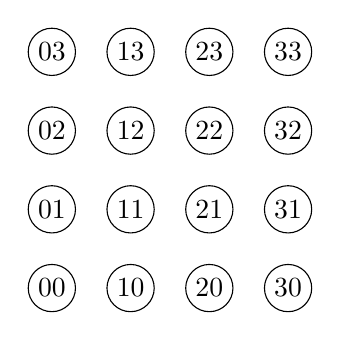
\begin{tikzpicture}
\centering
    \foreach \x in {0,...,3}
    \foreach \y in {0,...,3}
    \draw (\x,\y) circle (0.3) node {\x\y};

\end{tikzpicture}

\subsection{Testing the dsPIC33E microcontroller}

\begin{itemize}
\item The dsPIC series are a family of 16 bit microcontrollers which contain special instructions for performing more intensive mathematical operations. Some of them come in surface mount packages, but some are also DIP and will go on a breadboard (e.g. dsPIC33F). We can probably prototype initially using a dsPIC33E (which we have) and then port the code to the dsPIC33F (which hopefully shouldn't be too hard).
\item Tested $2^{15}$ $2\times 2$ real matrix multiplications at 12MHz. The operation involved about 16 instructions and took under 0.1s.
\item Created a one qubit simulator in C -- it can do the H, X and Z gates, mapped to buttons on the development board. The three lights are used to display the 0, 1, + and - states. Next steps -- extend to complex number arithmetic and multiple qubits
\item Tried the same $2\times 2$ matrix multiplication test, which takes significantly longer in C. There might be a way of making it faster, or just embedding assembly language.
\end{itemize}

\section{Two qubit tests}

There are 4 states for each qubit, $\ket{0}, \ket{1}, \ket{+}, \ket{-}$, we think there
are less than $3^3$ states for two qubits which means we can test a two qubit operation
with the 3 LEDs.

$ b_1 b_2 b_3$
qubit 1 is button 1, qubit 2 is button 2, button 3 is the two-qubit gate.

\begin{itemize}
    \item Choose a qubit
    \item choose a gate
\end{itemize}

decoding will use \textit{On, Off, Flashing} 
\end{document}
